\documentclass{zsarticle}

\usepackage{csquotes}

% --------------------------------------------------------------------
% Metadata
% --------------------------------------------------------------------

\pdfauthor{Jane Doe and John Smith}
\pdftitle{ZS style sheet and template}
\pdfkeywords{style sheet, template, Zeitschrift für Sprachwissenschaft}

\zsvolume{XX}
\zsissue{Y}
\zsarticle{Z}
\zsyear{2026}
\zsdoi{10.1515/zfs-YYYY-200Z}
\zsreceived{month year}
\zsaccepted{month year}
\zspublished{month year}
\zscitation{Doe, Jane \& John Smith. 2026. ZS style sheet and template: Publication guide in article form. \textit{Zeitschrift fuer Sprachwissenschaft} XX(Y).}

\title[ZS style sheet]{ZS style sheet and template}
\subtitle{Publication guide in article form}
\author[Doe \& Smith]{Jane Doe \and John Smith}

\affiliation{Author name(s) (corresponding author), University of A, Country, email(s)}
\affiliation{Author name(s), University of B, Country, email(s)}
\affiliation{Author name(s), University of C, Country, email(s)}
\keywords{style sheet, template, linguistic examples, citation, references}

\addbibresource{zs.bib}

\begin{document}

\maketitle

\begin{abstract}
Research articles must have the main text prefaced by an abstract of no more than 200 words summarizing the main arguments and conclusions of the article. In order to be interpretable on its own, the abstract should not contain in-text citations or uncommon abbreviations prior to their introduction in the main text. This document serves both as a style sheet and as a template for contributions to the \textit{Zeitschrift für Sprachwissenschaft} (ZS). It illustrates the formatting conventions, document structure, and environments available in the \texttt{zsarticle} class.
\end{abstract}

% ====================================================================
\section{Introduction}\label{sec:intro}
% ====================================================================

The \textit{Zeitschrift für Sprachwissenschaft} (ZS) welcomes manuscripts in English and German presenting current, original research results that have not been submitted or published elsewhere. Authors are responsible for the grammatical and orthographic correctness of their submission. Article manuscripts should not exceed 10,000 words or 37 pages.

This style sheet provides details on the design of text parts (\Secref{sec:textstyle}), addresses citation and references (\Secref{sec:citation}), covers orthographical conventions (\Secref{sec:ortho}), and discusses the handling of statistical data (\Secref{sec:stats}). \Secref{sec:reviews} contains a note on reviews, \Secref{sec:font} introduces the Libertinus font family, and \Secref{sec:latex} provides guidance on using this \LaTeX{} template.

% ====================================================================
\section{Text-structure style}\label{sec:textstyle}
% ====================================================================

The ZS style is based on the proposal for \enquote{text-structure style} in \textit{The Generic Style Rules for Linguistics}. This section describes general and linguistic conventions on parts of an article. \Secref{sec:sections} is on sections, \Secref{sec:examples} on linguistic examples, followed by tables and figures in \Secref{sec:tabfig}, the use of font for highlighting (\Secref{sec:emphasis}), and abbreviations (\Secref{sec:abbrev-sec}).

% --------------------------------------------------------------------
\subsection{Sections}\label{sec:sections}
% --------------------------------------------------------------------

Each section and possibly subsection of the body of an article has a heading. While headings start with a capital letter, they do not internally feature special capitalization. Words following colons within headings usually begin with a small letter.

Sections and subsections are consecutively numbered, beginning with Section~1 (the introduction). More than three section levels are rarely helpful. If a fourth level is necessary, unnumbered intermediary headings are used:

\paragraph{Unnumbered heading} This is a fourth-level heading, set in Libertinus Sans at 11\,pt bold, without a number. It is used only when strictly necessary.

If cross references to individual numbered sections, appendixes, tables, figures, or footnotes occur, these terms are not abbreviated. If the number follows, the term is capitalized:

\begin{zsquote}
see \Figref{fig:questions} and \Footref{fn:sample}; see the analysis in the next section and data in the appendix
\end{zsquote}

% --------------------------------------------------------------------
\subsection{Linguistic examples}\label{sec:examples}
% --------------------------------------------------------------------

Italics indicate exemplary linguistic material. If linguistic material in the running text is from another language, a translation in single curly quotation marks follows immediately:

\begin{zsquote}
[\ldots] everything is given and salient except for \objlang{reparieren} \translation{repair} [\ldots]
\end{zsquote}

In numbered examples such as \ref{ex:glauben}, the translation in single curly quotation marks follows in a separate line:\footnote{This is the sample footnote referred to later.\label{fn:sample}}

\ex.\label{ex:glauben} \objlang{Du wirst es nicht glauben.}\\
\translation{You will not believe it.}

If interlinear glossing is provided, each word in the example is aligned with its literal translation. Where relevant, morphemic glossing follows the rules described in \textit{The Leipzig Glossing Rules}. The source language can be given in round brackets after the example in italics, as in \ref{ex:icelandic1}. Alternatively, the source language can be given on a line preceding the example, as in \ref{ex:icelandic2}.

\ex.\label{ex:icelandic1}
\gll Storm-ur-inn rak b\'{a}t-inn \'{a} land. \hfill (\textit{Icelandic})\\
storm-\textsc{nom}-\textsc{def} drove boat-\textsc{acc}-\textsc{def} on land\\
\glt \translation{The storm drove the boat ashore.}

\ex.\label{ex:icelandic2} \textrm{Icelandic}\vspace{-0.5\baselineskip}
\gll Storm-ur-inn rak b\'{a}t-inn \'{a} land.\\
storm-\textsc{nom}-\textsc{def} drove boat-\textsc{acc}-\textsc{def} on land\\
\glt \translation{The storm drove the boat ashore.}

Boldface can highlight expressions of interest within numbered examples, see~\ref{ex:sub:a}; small caps conventionally indicate focused expressions, see~\ref{ex:sub:b}.

\ex.\label{ex:sub}
\a.\label{ex:sub:a} \objlang{The storm drove \textbf{the boat} ashore.}
\b.\label{ex:sub:b} \objlang{The storm drove the boat} \focus{ashore}\objlang{.}

A preceding asterisk indicates an ungrammatical example, and the intended meaning can be given in round brackets, see~\ref{ex:ungram}:

\ex.\label{ex:ungram} *\objlang{The storm drived the boat ashore.}\\
(\translation{The storm drove the boat ashore.})

Each numbered example must be referred to in the running text. Adding \enquote{Example} before a bracketed example number is not necessary and not desired by the ZS.

% --------------------------------------------------------------------
\subsection{Tables and figures}\label{sec:tabfig}
% --------------------------------------------------------------------

Like numbered examples, tables and figures are numbered consecutively and must be mentioned in the running text. Paragraphs before tables and figures do not finish on a colon because tables and figures may shift to another position. Tables and figures must feature captions. Captions of tables appear above the table, captions of figures appear below the figure.

Fonts in tables, graphics, and illustrations: please use the font Libertinus Sans (a sans-serif variation of the Libertinus family, see \Secref{sec:font}) instead of the standard Libertinus Serif in tables and figures as well as captions. The standard font size in tables is 11\,pt, which can be reduced to 10\,pt (as in captions) or 9\,pt (as in footnotes).

\Tabref{tab:nouns} shows the frequency of some English nouns.

\begin{table}[ht]
\begin{threeparttable}
\caption{Frequency of some English nouns (BNC)\tnote{a}}\label{tab:nouns}
\begin{tabular}{llrlr}
\toprule
\tablehead{Singular\tnote{b}} & & \tablehead{Plural} & & \tablehead{\% of singular}\\
\midrule
person & 24671 & persons & 4034 & 86\,\%\\
house  & 49295 & houses  & 9840 & 83\,\%\\
hare   & 488   & hares   & 136  & 78\,\%\\
\bottomrule
\end{tabular}
\begin{tablenotes}
\item[a] Data and, partially, table layout are taken from The Generic Style Rules for Linguistics (p.~9).
\item[b] Headers usually begin with capital letters. Footnotes in tables appear below the table and use letters for reference, not numbers.
\end{tablenotes}
\end{threeparttable}
\end{table}

On graphics and figures: figures and graphics serve to illustrate (quantitative) data. It is essential to consider the balance between tabular and visualized information within texts. The ZS is published exclusively in digital form, eliminating restrictions regarding the use of colour. Nevertheless, it is essential to ensure readability and inclusivity for readers with colour perception difficulties \parencite{cramerietal2020,cramerietal2024}. \Figref{fig:questions} shows a sample figure.

\begin{figure}
\centering
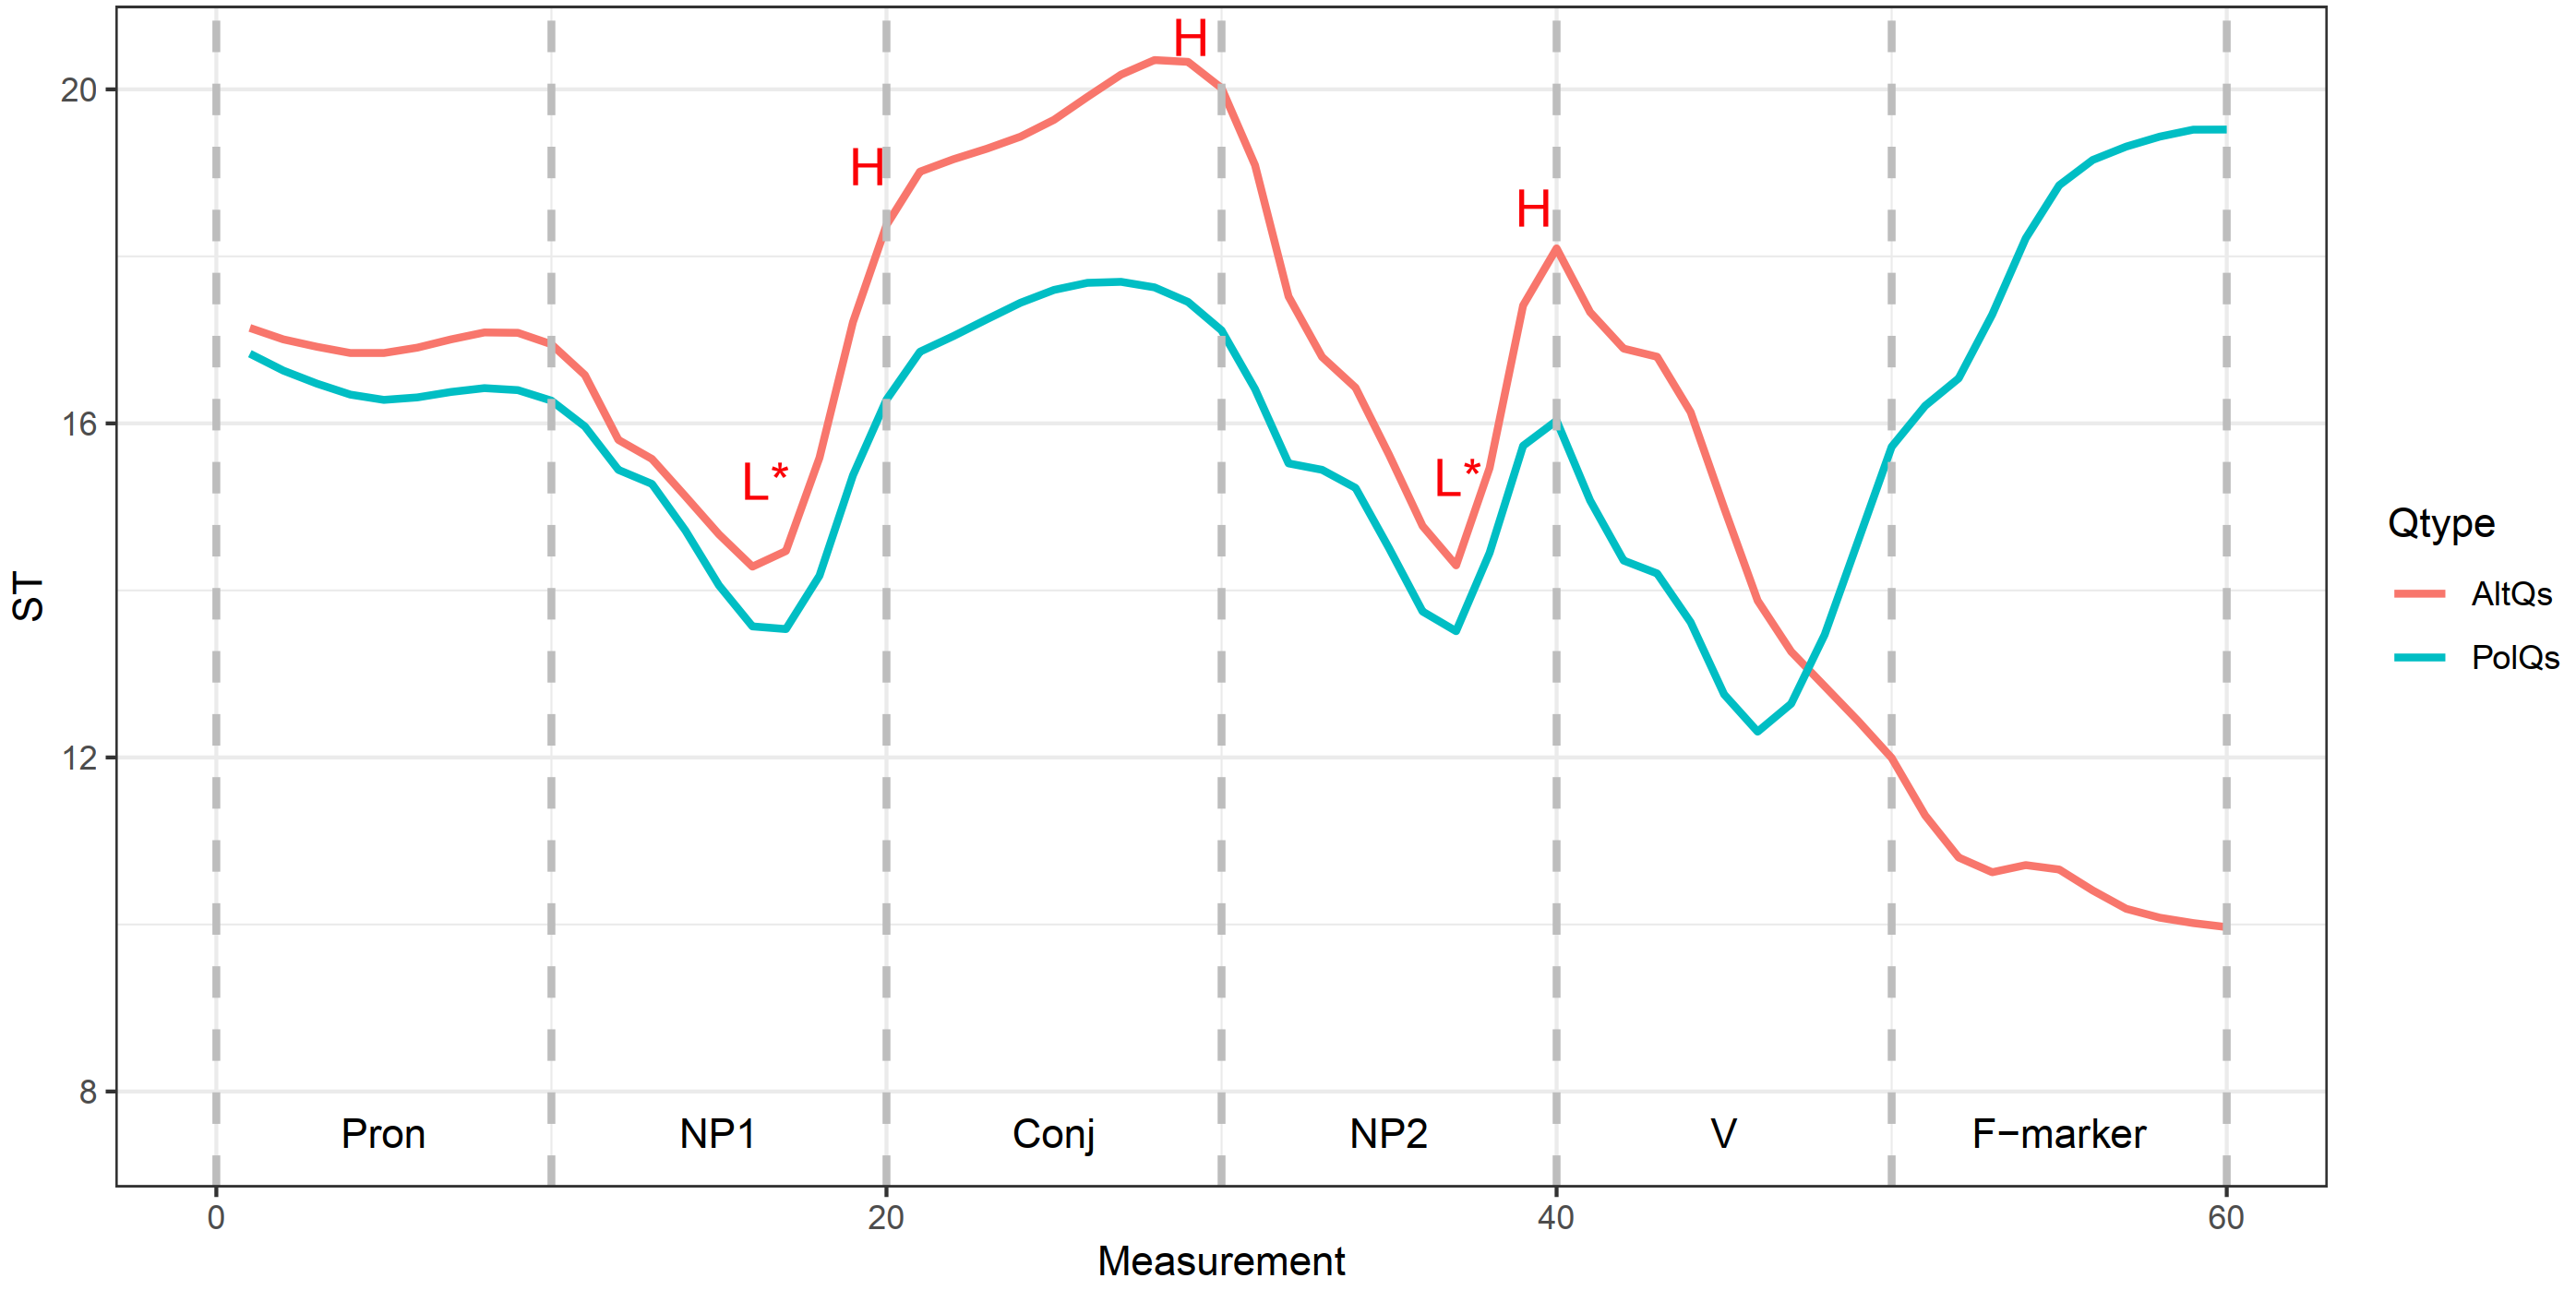
\includegraphics[width=0.85\textwidth]{questions}
\caption{Semitone (ST) trajectories for alternative questions (AltQs) and polar questions (PolQs)}\label{fig:questions}
\end{figure}

For article production, authors are required to submit image files separately. Figures should be numbered sequentially, and the file name should match the reference in the text (e.g.\ \texttt{figure\_1.jpg} for \Figref{fig:questions}). Preferred formats are vector-based (SVG, PDF, EPS) for diagrams and pixel-based (JPEG, TIFF, at least 300\,dpi) for photographs.

% --------------------------------------------------------------------
\subsection{Typographical means of emphasis: italics, boldface, and small caps}\label{sec:emphasis}
% --------------------------------------------------------------------

Special formatting should be used minimalistically. Italics are used:
\begin{itemize}
\item for linguistic examples in running text or numbered example environments;
\item for book, journal, and film titles;
\item for metalinguistic reference to technical terms (e.g.\ \enquote{calling these lexemes \term{discourse} rather than \term{modal particles}});
\item for emphasis in general (\enquote{is \emph{only} true if});
\item for introduction or intermittent emphasis of key terms, concepts, principles, etc.
\end{itemize}

Boldface can highlight expressions of interest within linguistic examples, see~\ref{ex:sub:a} in \Secref{sec:examples}. Underlining should only be used exceptionally. All caps, quotation marks, or capitalization are not used for highlighting. Small caps are reserved for abbreviations of grammatical categories in glossing and stress or focus in example sentences, see~\ref{ex:sub:b}.

% --------------------------------------------------------------------
\subsection{Abbreviations}\label{sec:abbrev-sec}
% --------------------------------------------------------------------

Abbreviations can be helpful if they are common or reduce a complex uncommon term (CUT) that a text refers to frequently. An alphabetical list of abbreviations can be provided in a designated section; for illustration, see the Abbreviations section below.

% ====================================================================
\section{Citation and references}\label{sec:citation}
% ====================================================================

The ZS adopts suggestions on citation and references from \textit{The Generic Style Rules for Linguistics} while mostly retaining the reference style proposed in \textit{The Unified Style Sheet for Linguistics}. \Secref{sec:citing} is on citing and quoting, \Secref{sec:refsection} is on references.

% --------------------------------------------------------------------
\subsection{Citation and quotations}\label{sec:citing}
% --------------------------------------------------------------------

Bibliographical sources appear as narrative or parenthetical citations in the running text, consisting of author surname(s), year, and page(s). If the surname features a prefix like \emph{van} or \emph{De}, the prefix is present in the citation:

\begin{zsquote}
[\ldots] as \textcite[125--126]{vangelderen2022} argues [\ldots]
\end{zsquote}

In parenthetical citations, author names appear in the round brackets as well, separated from the year by a space:

\begin{zsquote}
[\ldots] not yet clear (for an overview, see \cite{vangelderen2022}).
\end{zsquote}

The names of a pair of authors are conjoined by an ampersand. In case of more than two authors, the first author's name is followed by \emph{et~al.}:

\begin{zsquote}
\parencite{crainetal1986}; \parencite{blasietal22}
\end{zsquote}

Citations following quotations in the running text appear after the closing quotation marks and before a (final) punctuation mark:

\begin{zsquote}
\enquote{[\ldots] everything in the clause is given} \parencite[63]{vangelderen2022}.
\end{zsquote}

Longer quotations should appear in a separate indented block, in which case quotation marks are omitted and the source is cited in brackets after the final punctuation mark:

\begin{zsquote}
The second factor is the learner's need to be exposed to one or more languages (spoken or signed) to build the lexicon and to become familiar with interface constraints [\ldots]. Lexical differences are responsible for all cross-linguistic variation, and parameters are now only relevant to that domain [\ldots]. \parencite[3]{vangelderen2022}
\end{zsquote}

% --------------------------------------------------------------------
\subsection{The section References}\label{sec:refsection}
% --------------------------------------------------------------------

Each source in the reference section must be referred to in the main text or a footnote. The reference section may not include entries on further reading if the sources in question are not also mentioned elsewhere.

References are ordered alphabetically according to author name(s). The complete surname of the first author is given first, followed by a comma and the given name in full form. All co-authors' names appear in their natural order. The ampersand conjoins the last of two or more names.

The following examples illustrate the main reference types. A journal article entry \parencite{blasietal22} presents the article title in roman font with sentence case. The journal title follows in italics with title case. Only a space separates journal title and volume number. An en dash separates first and last page numbers.

An article in an edited volume \parencite{cristofaro2017} presents full information on the edited volume after the word \emph{In}. An edited volume \parencite{cangemietal2018} differs from a monograph only by the addition of (eds.) after the names. A monograph \parencite{vangelderen2022} follows the same pattern.

Reprints show the original year in square brackets \parencite{weinhold1883}. Theses are presented like monographs with a university as the publisher \parencite{sahlgren2006}. Online sources \parencite{native2025,r2021} may feature an access date. Proceedings contributions \parencite{crainetal1986} are presented like journal articles. Conference papers \parencite{faller2019} provide event information after the title.

% ====================================================================
\section{Orthographical conventions}\label{sec:ortho}
% ====================================================================

For consistent spelling, the ZS refers to the Oxford English Dictionary or Merriam-Webster. Grammar and punctuation rules should be consistent.

% --------------------------------------------------------------------
\subsection{Punctuation}\label{sec:punctuation}
% --------------------------------------------------------------------

In the interest of consistency, the ZS adopts the following conventions.

\subsubsection{Hyphens and dashes}\label{sec:dashes}

In hyphenating compound modifiers (\emph{spatialization-of-form hypothesis}), we recommend following Oxford conventions. The ZS employs the hyphen, rather than the en dash, in expressions like \emph{editor-author relationship}.

En dashes introduce entries in vertical lists. Unspaced en dashes indicate ranges: pp.~23--31. The ZS uses spaced en dashes as parenthetical dashes:

\begin{zsquote}
The ZS employs spaced en dashes~-- rather than unspaced em dashes, which are twice as long and uncommon in some languages~-- as parenthetical dashes.
\end{zsquote}

\subsubsection{Quotation marks}\label{sec:quotes}

Please use curly quotation marks and apostrophes. Quotations are in double quotation marks, quotations in quotations are in single quotation marks:

\begin{zsquote}
Illustrating that \enquote{all conventionally implicated content is assigned \enquote*{the same semantic force as a main clause}}, the paper supports \citeauthor{potts2005}'s (\citeyear{potts2005}) insight [\ldots]
\end{zsquote}

Single quotation marks are also used for translations of exemplary linguistic material, see \Secref{sec:examples}.

% --------------------------------------------------------------------
\subsection{Capitalization}\label{sec:capitalization}
% --------------------------------------------------------------------

Internal capitalization of lexical words, i.e.\ title case, applies to expressions that can be regarded as proper names: conferences, journal titles, and book series. When a part of a text is referred to individually, the expression features an initial capital letter (in \Secref{sec:examples}, \Footref{fn:sample}, \Tabref{tab:nouns}, \Figref{fig:questions}).

Capitalization should be used only if absolutely necessary. In particular, title case should not be used for hypotheses, principles, theories, etc.:\ \emph{the minimalist program}, \emph{word-space model}, \emph{the spatialization-of-form hypothesis}.

% ====================================================================
\section{Handling statistical data}\label{sec:stats}
% ====================================================================

In general, we recommend following the guidelines of the American Psychological Association (APA) regarding the presentation of statistical data.

We recommend rounding normal interval- or ratio-scaled data in tabular representation to a maximum of two decimal places. Exact $p$-values should be reported to three decimal places in the form $p = .006$. Otherwise, standard significance codes can be used, as applied in R \parencite{r2021}, see \Tabref{tab:sigcodes}.

\begin{table}
\caption{Standard significance codes as applied in R}\label{tab:sigcodes}
\begin{tabular}{ll}
\toprule
\tablehead{Code for significance} & \tablehead{$p$-value range}\\
\midrule
{***} & {[0, 0.001]}\\
{**}  & {(0.001, 0.01]}\\
{*}   & {(0.01, 0.05]}\\
{.}   & {(0.05, 0.1]}\\
      & {(0.1, 1]}\\
\bottomrule
\end{tabular}
\end{table}

What and how statistical data is reported depends on the research question. We refer to recommendations such as those by \textcite{levshina-2015} or \textcite{norrisetal-2015}. We advise that statistical analyses be described in the main text in a way that allows readers with less statistical knowledge to understand the results.

A basic description of the data is important, at the very least indicating the number of data points, measures of central tendency (e.g.\ median, mean), and measures of variability (especially standard deviation).

Furthermore, we encourage the complete sharing of materials, data, and scripts, for example, via OSF. We also recommend reporting 95\,\% confidence intervals and effect sizes \parencite[see][]{bodo2019}.

% ====================================================================
\section{A note on reviews}\label{sec:reviews}
% ====================================================================

Contributions titled \emph{Book review} feature details on the reviewed volume in their subtitle, in four parts separated by periods: name(s), title, publisher information, and pages. Names are presented in boldface in their native order.

% ====================================================================
\section{Font: Libertinus}\label{sec:font}
% ====================================================================

ZS contributions use the non-proprietary typeface family Libertinus, most prominently the fonts Libertinus Serif for running text and Libertinus Sans for some special environments like titles, headings, tables, and annotations in figures. This typeface family is freely available under an open-access license. When using this \LaTeX{} template, the Libertinus fonts are loaded automatically via the \texttt{fontspec} package; authors only need to ensure that the fonts are installed on their system.

% ====================================================================
\section{Document formatting in \LaTeX}\label{sec:latex}
% ====================================================================

This template provides the \texttt{zsarticle} document class, which sets up all formatting automatically. The class requires Lua\LaTeX{} (preferred) or Xe\LaTeX{} and uses \texttt{biblatex} with the \texttt{langsci-unified} style.

% --------------------------------------------------------------------
\subsection{Class options}\label{sec:options}
% --------------------------------------------------------------------

The class supports the following options:
\begin{itemize}
\item \texttt{submission} -- produces an anonymized version for double-blind review (author names and affiliations are hidden);
\item \texttt{final} -- produces the final published version with copyright notice.
\end{itemize}

The default mode (no option) produces a draft with full citation and license information in the first-page footer.

% --------------------------------------------------------------------
\subsection{Front matter commands}\label{sec:frontmatter}
% --------------------------------------------------------------------

The preamble should define the following metadata:
\begin{itemize}
\item \verb|\title[short title]{Full title}| -- the optional argument sets the running head;
\item \verb|\subtitle{Subtitle}| -- article subtitle;
\item \verb|\author[short author]{Author names}| -- use \verb|\and| between authors;
\item \verb|\affiliation{...}| -- one call per author with name, department, university;
\item \verb|\correspondence{name, \email{...}}| -- corresponding author;
\item \verb|\keywords{...}| -- displayed after the abstract.
\end{itemize}

Journal metadata is set with \verb|\zsvolume|, \verb|\zsissue|, \verb|\zsarticle|, \verb|\zsyear|, \verb|\zsdoi|, \verb|\zsreceived|, \verb|\zsaccepted|, and \verb|\zspublished|.

% --------------------------------------------------------------------
\subsection{Environments and helpers}\label{sec:environments}
% --------------------------------------------------------------------

The class provides several environments and commands:
\begin{itemize}
\item \texttt{abstract} -- for the abstract, with automatic keyword display;
\item \texttt{zsquote} -- for indented block quotations (10\,pt, indented on both sides);
\item \texttt{acknowledgements} -- for the acknowledgements section;
\item \texttt{funding} -- for funding information;
\item \texttt{abbreviations} -- for the list of abbreviations;
\item \verb|\term{}|, \verb|\objlang{}|, \verb|\focus{}|, \verb|\translation{}| -- semantic formatting;
\item \verb|\Secref{}|, \verb|\Figref{}|, \verb|\Tabref{}|, \verb|\Footref{}|, \verb|\Appref{}| -- cross-reference helpers.
\end{itemize}

% --------------------------------------------------------------------
\subsection{Building the document}\label{sec:building}
% --------------------------------------------------------------------

Compile with:
\begin{verbatim}
latexmk -lualatex main.tex
\end{verbatim}

Or manually:
\begin{verbatim}
lualatex main.tex
biber main
lualatex main.tex
lualatex main.tex
\end{verbatim}

% ====================================================================
% Back matter
% ====================================================================

\begin{acknowledgements}
We thank the editorial team for their support.
\end{acknowledgements}

\begin{funding}
This research received no external funding.
\end{funding}

\begin{abbreviations}
\begin{tabular}{@{}ll@{}}
APA & American Psychological Association\\
CUT & complex uncommon term\\
SI  & Syst\`eme international d'unit\'es `International System of Units'\\
ZS  & \textit{Zeitschrift für Sprachwissenschaft}: Journal of the Linguistic Society of Germany
\end{tabular}
\end{abbreviations}

\appendix
\section{A sample appendix}\label{app:sample}

This appendix exists so that \Appref{app:sample} resolves to a live cross-reference example. Appendixes follow the abbreviations and precede the references.

\printbibliography

\end{document}
